\documentclass[a4paper]{article}
\usepackage{color,epsfig}
\usepackage{makecell}
\newcolumntype{C}[1]{>{\centering\arraybackslash}m{#1}}
\usepackage{array}
\usepackage{longtable}
\usepackage{afterpage}
\usepackage{mdframed}
\usepackage{listings}
\usepackage{dirtytalk}
\usepackage{amsmath}
\newcommand{\pdif}[2]{\frac{\partial #1}{\partial #2}}
\newcommand{\oline}[1]{ \overline{#1}}
\definecolor{Olivegreen}{rgb}{0,.4,0}
\renewcommand{\lstlistingname}{\bfseries\textcolor{black}{Table}}% Listing -> Algorithm

\begin{document}

{\Large \bf {Response to Referee 1}}
\vspace{1cm}

{\textcolor{Olivegreen}{
We appreciate the constructive critique from the reviewer. We have carefully examined all the concerns and here are the answers to them. We believe these changes have improved the quality of the manuscript.
}}


\begin{enumerate}
%.................................................................
\item
\textit{As the paper essentially concerns the methodology of decomposition techniques for advection dominated-flows, it is not obvious to me that it fits the scoop of Chemical Engineering Science. For this reason I think the authors should introduce what could be the benefit of ``data-driven decomposition techniques''for the problem of interest for CES and elaborate on the goal of the DMD / POD in that context. In the same spirit, to better understand the possible advantages of the decomposition, the authors could synthesis how compressed is the information to reproduce that dynamic with respect to the original database.}
\vspace{.2cm}

We understand the reviewer’s concern about clarifying the relevance of data-driven decomposition techniques for rising-bubble problems within the scope of Chemical Engineering Science, and we also acknowledge the need to show how efficiently these methods compress the original database while retaining the essential dynamics. 

The effectiveness of decomposition techniques lies in the physical insights obtained from the extracted modes and their temporal coefficients in POD, as well as their frequency content in DMD—an analysis that is planned for future work. In the longer term, the objective is to conduct an in-depth mode analysis to investigate complex dynamical features of rising bubbles, such as the onset of wake instability that is critical in transport phenomena. As an essential first step toward this goal, we needed to determine which decomposition method and which frame of reference yield the lowest-rank representation of the full dataset. A lower number of modes is naturally preferred, as it enables a more tractable and focused physical interpretation. In line with this motivation, we began by examining two classical decomposition techniques (POD and DMD) to identify the minimal number of modes required to represent the dynamics before proceeding to a detailed mode analysis. To further clarify the goal and the relevance of these techniques for the readers in the community of Chemical Engineering Science, the following explanations are given in the Introduction on \textbf{page 2, Lines:26-30 and 55-56}:

\textcolor{blue}{P2. L26-30: In the context of a rising bubble, these techniques can provide a low-order representation of complex bubble dynamics—such as wake instabilities—through an in-depth analysis of the extracted modes. Depending on the flow regime and the level of complexity, the number of modes required to represent the full dynamics can vary substantially, and selecting an appropriate decomposition method that yields the fewest possible modes remains a persisting challenge.}

\textcolor{blue}{P2. L55-56: The findings of this paper can be used as a roadmap for mode analysis by identifying an efficient decomposition method that uses a small number of modes.}

Regarding the question of dimensionality reduction and information compression, our results show that for the 3D bubble case $C_5$ as the most complex case with 690 snapshots, a maximum of 15 modes is sufficient to accurately represent the full dataset, corresponding to a compression ratio of 46. This compares favorably with the work of Yin et al. (2023), where 30 modes were used to represent 140 snapshots of a deformed bubble, resulting in a compression ratio of roughly 4.6. This information is added on \textbf{page 17, Lines:386-389} as follows:

\textcolor{blue}{P17. L386-389: In particular, the rise characteristics of the 3D bubble $C_5$, as the most complex case with 690 snapshots, were estimated using 15 modes, yielding a compression ratio of 40. This is notably less than the number of modes used by Yin et al.(2023), who employed 30 modes to represent 140 snapshots, resulting in a compression ratio of approximately 4.6.}


\item
\textit{I found that the description of the methodology to obtain the mode decomposition (which is the core of the paper) is not clear and misleading. First the use of the name ``semi-Lagrangian'' corresponds, to my understanding, to an Eulerian description in a sub-domain following (i.e. translated) the center of mass of the bubble, whereas the name ``Lagrangian'' actually corresponds to the ``semi-Lagrangian'' name of the original paper of Yin et al. 2023 Chem. Eng. Research and Design.}
\vspace{.2cm}

We greatly appreciate the reviewer’s critical perspective on the description of the frames used in this work. 

As correctly mentioned by the reviewer, the ``Semi-Lagrangian'' frame corresponds to a sub-domain of the Eulerian grid moving with the center of mass of the bubble. On the other hand, the ``Lagrangian'' frame consists of tracking fluid particles initially introduced in the Eulerian frame which is consistent with the ``Lagrangian'' frame considered in the work of Yin et al. (2023). To avoid any confusion, the name ``Semi-Lagrangian'' is now changed to ``Moving-Eulerian'' frame in the revised manuscript and all the Figures are updated with the new abbreviations. The letters ``SL'' are now replaced with ``ME'' representing the ``Moving-Eulerian'' frame throughout the entire manuscript and all the figures.


\item
\textit{Further, the use of the DMD in the case of the Lagrangian case, and the so-called semi-Lagrangian case (following the terminology of the present paper) are not clearly explained. In the previous papers on the subject, in the Lagrangian framework, in addition to the set of values at the Lagrangian point, it was necessary as well to consider the set of coordinates of the Lagrangian points in the input data. In the present paper, there is absolutely no mention of how these Lagrange coordinates are used. I thus cannot understand how the bubble shape or trajectory of the bubble center can even be reconstructed.}
\vspace{.2cm}


Thanks to the reviewer for the precise and critical evaluation of coordinates of the Lagrangian and Semi-Lagrangian data points.

As correctly noted by the reviewer, both the Semi-Lagrangian and Lagrangian data points will have a different set of coordinates at every time step that must be considered. More accurately, the coordinates are decomposed and reconstructed separately in addition to the velocity and other observation variables to determine the interface and other rise characteristics. In the revised manuscript, it is shown that the matrix of position, denoted as $P$, contains the coordinates of the Lagrangian particles and the Semi-Lagrangian grid points in the corresponding frame of reference. The matrix of position contains twice as many rows as the gas volume fraction field in the 2D axisymmetric case, and three times as many rows in the 3D Cartesian case. The cumulative energy criterion for the matrix of position shows that it is inherently low-rank and can be accurately reconstructed using only a single mode. To better address the use of coordinate points and their reconstruction, we have added \textbf{Figure B1} and updated \textbf{Figure B2} in \textbf{Appendix B}, which provide a more detailed description of the input data of each frame and the cumulative energy of the Lagrangian and Eulerian coordinates as follows:

\appendix
\setcounter{section}{1}

\section{\textcolor{blue}{Input and output observation values of data-driven methods and rank selection}}
\label{Append_B}

\renewcommand{\theequation}{B.\arabic{equation}}
\setcounter{equation}{0}

\textcolor{blue}{The input and output data matrices for different frames of reference with their corresponding observation values are schematically shown in Fig.\ref{Fig9}. Rise velocity, the shape of the bubble and its centroid are the main characteristics studied in the present work. Thus, the upward component of the velocity and the gas volume fraction fields are considered. In the Lagrangian and moving-Eulerian frames of reference, the set of coordinates of Lagrangian tracers and moving-Eulerian grids should also be obtained during the rise process. Therefore, in these two frameworks, the coordinate matrix of the data points is also decomposed and later reconstructed. Obviously, the coordinates of the fixed Eulerian grid do not change and thus require no reconstruction. For the selected frame, the input data matrices of velocity ($V$), gas volume fraction ($G$), and coordinates ($P$) in stacked form are separately decomposed, and later a truncated representation using $r$ modes is reconstructed as $V'$, $G'$, and $P'$. In this way, both the shape and the velocity field are represented in the selected frame at their corresponding coordinate. The size of the input matrix varies in the number of rows depending on the number of data points and the number of components for each observation value. For example, the input matrix $G$ in the Eulerian frame for bubble C$_3$, with $m=400$ snapshots and a grid size of $n_r=250$ and $n_z=750$, is of size $(250 \times 750) \times 400$. For the same case in the Lagrangian frame, the $P$ matrix has the same number of columns with $n_s= (2\times250 \times 750)$ rows because it contains both components of the coordinates. It should be noted that, due to the scattered output of Lagrangian tracking, an interpolation of the scattered data points onto a uniform grid is required to represent the bubble interface, whereas the Eulerian and moving-Eulerian frames are already defined on their original uniform grids.}


\begin{figure}[h]
	\centering
	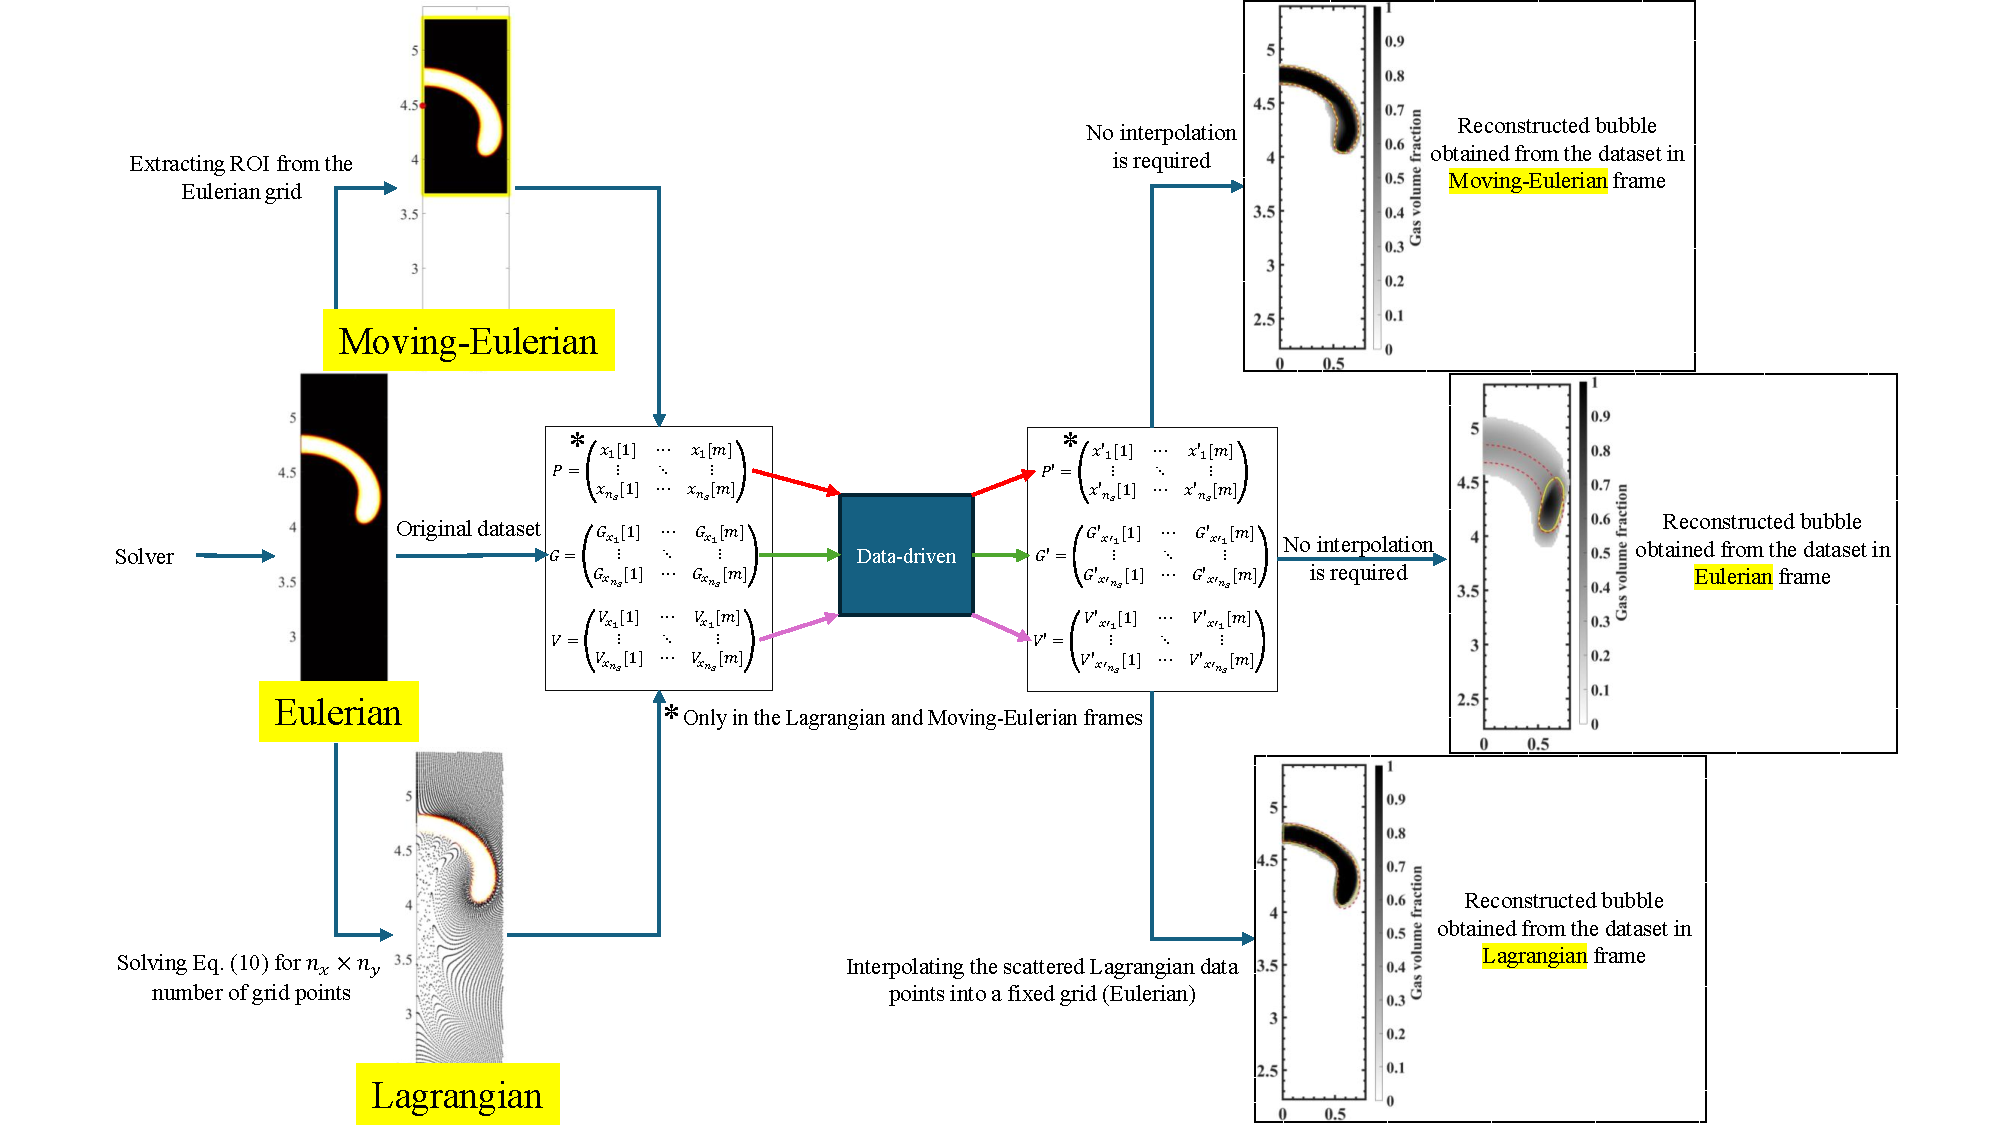
\includegraphics[scale=0.45,trim={1.8cm 00cm 1cm 0cm},clip]{Figure_B.1.pdf}
	\caption{\textcolor{blue}{Schematic of input and output data matrices of data-driven methods.}}
	\label{Fig9}
\end{figure}


\textcolor{blue}{It is worth mentioning that for the coordinate matrices of Lagrangian particles and the moving-Eulerian frame, the cumulative energy criterion reaches 99\% with only 1 mode, reflecting the inherently low-rank/compact structure of particle positions compared to the more dispersive velocity and gas volume fraction fields. Thus, a single-mode reconstruction is considered for the coordinates of the Lagrangian and moving-Eulerian data points unless otherwise specified.}
\begin{figure}[!t]
	\centering
	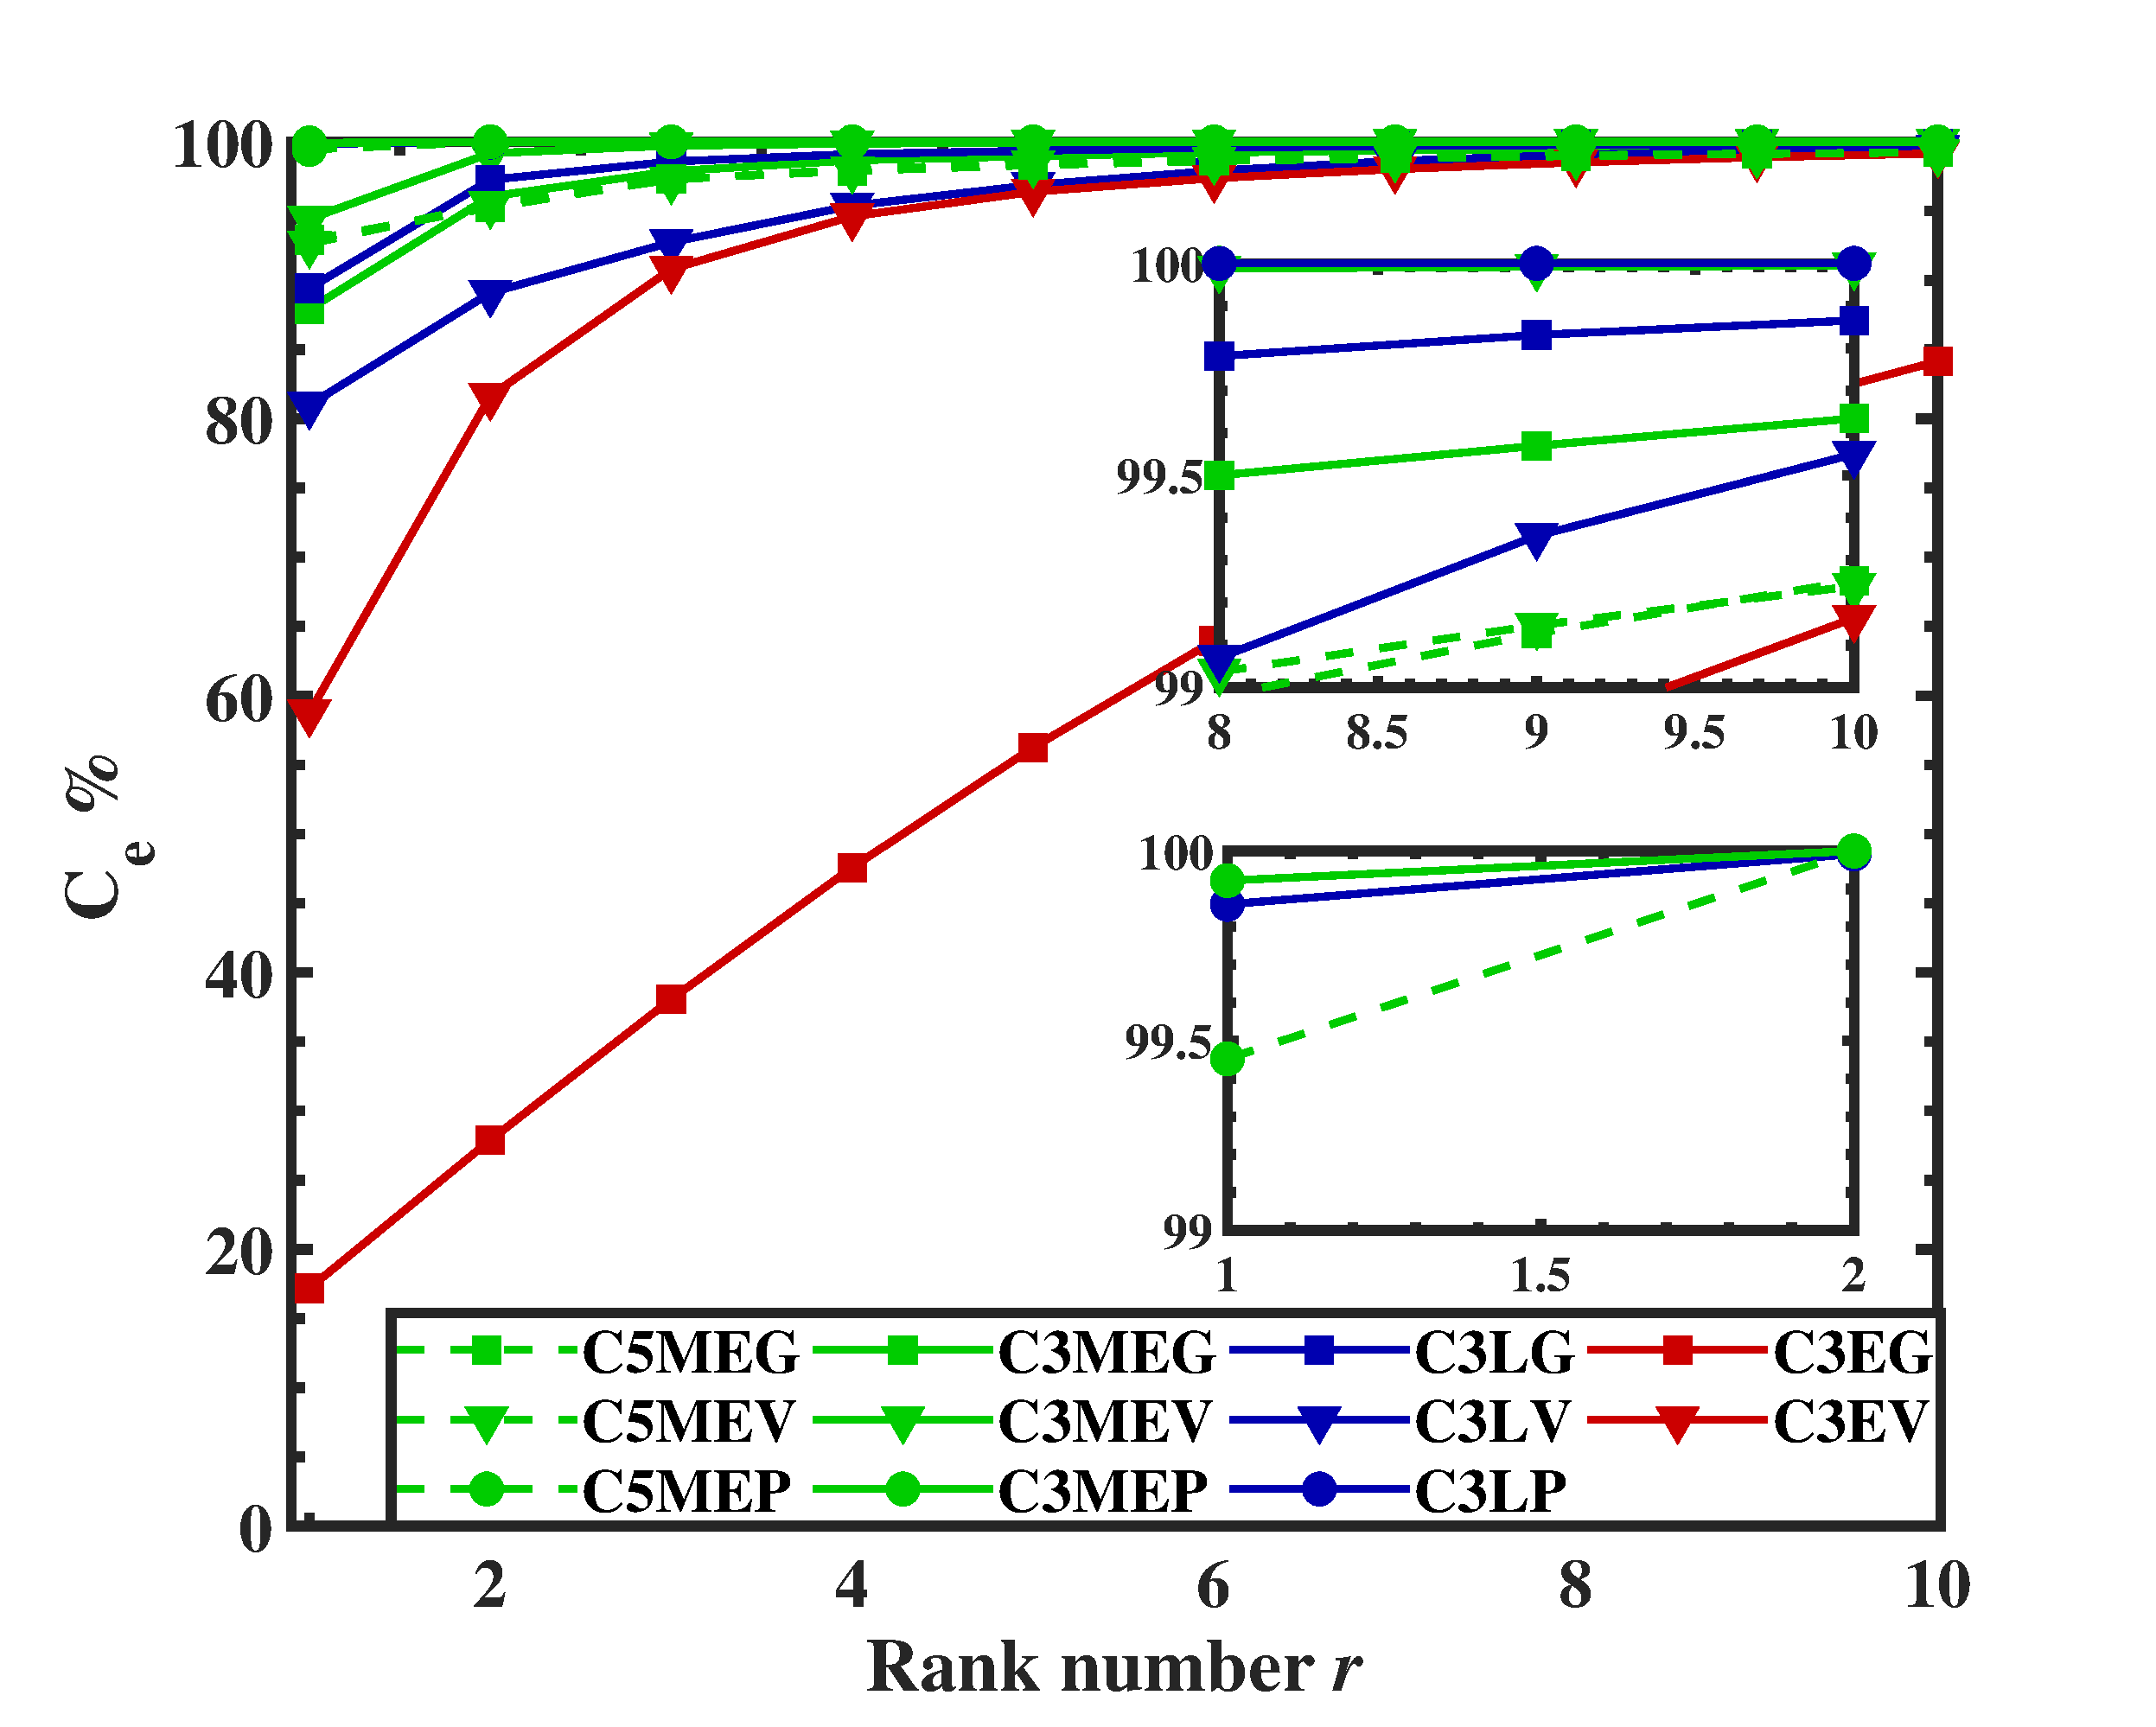
\includegraphics[scale=0.25,trim={00cm 00cm 0cm 0cm},clip]{Figure_B.2.eps}
	\caption{\textcolor{blue}{Rank selection based on the cumulative energy profile for bubble cases C$_5$ (dashed-line) and C$_3$ (solid line) within Eulerian (red), Lagrangian (blue), and moving-Eulerian (green) frameworks. Square, circle and triangle markers denote gas volume (G), upward velocity component (V) and coordinates datasets (P).}}
	\label{Fig10}
\end{figure}


\item
\textit{It is not clear what is done exactly when the authors use the velocity data for the mode decomposition. Are they considering only the vertical velocity or full vector fields with the 3 components (line 193)? And finally, why is the full dataset (volume fraction fields + velocity vector fields) not considered as an input case?}
\vspace{0.2cm}

Thanks for this fruitful comment. Regarding the velocity field, we clarify that only the vertical component was used in the decomposition. This choice is motivated by the focus of the present study on the rise velocity, which is primarily determined by the vertical component.

In response to why we did not considered the full dataset as an input case, as shown in \textbf{Section~5.1}, the gas-volume-fraction and velocity fields exhibit different levels of complexity, and combining them would substantially increase the number of modes required for accurate reconstruction compared to using a single field in the data matrix. In principle, each field (e.g., gas volume fraction, upward component of the velocity field, and the coordinate points in the Lagrangian and moving-Eulerian frames) is provided as a separate input and processed independently.

To further clarify these points, we have added \textbf{Figure~B1} in \textbf{Appendix B}, which schematically illustrates how the input matrices for each field are individually decomposed and reconstructed. Additionally, the description of the input data matrices on \textbf{page~9 Lines:197-204}  is revised as follows:

\textcolor{blue}{P9. L197-204: For brevity, the framework and the observation values are abbreviated as $\textit{E}$, $\textit{L}$, and $\textit{ME}$ for Eulerian, Lagrangian, and moving-Eulerian frameworks, followed by $\textit{G}$, $\textit{V}$ or $P$ which refer to gas volume fraction, upward component of the velocity field, and the coordinates of the data points, respectively. Here, only the upward (vertical) velocity component is used, as the rise velocity is determined exclusively by this component. Considering three frame of references, two decomposition methods and three observation values, there can be 18 combinations that can be defined. For instance, the decomposition of the upward velocity field in the Eulerian frame using the POD method is denoted as $\textit{EV-POD}$. Further details regarding the input and output data matrices are given in Appendix B.}


\item
\textit{I do not understand the following sentence on line 114: ``The dataset obtained from the trajectories of moving grid points is temporally low-dimensional compared to that of fixed Eulerian grid points.'' The number of degrees of freedom to describe the flow in a Eulerian or a Lagrangian setting should remain identical. Does it mean that there is a subsampling of the Lagrangian data from the Eulerian data? Further it is not said in the paper how many Lagrangian points are used. It is important to be sure that the comparison between the different data layouts for the mode decomposition is not biased.}
\vspace{.2cm}


Thank you for your constructive feedback. 


The fact that Lagrangian trajectories are temporally low-dimensional reflects their reduced temporal variability compared with the Eulerian frame. In other words, if each Lagrangian point is regarded as a moving probe in the flow, the recorded quantities exhibit less temporal fluctuation because the probe is advected with the fluid. In contrast, a fixed Eulerian probe samples different flow structures passing through its location, resulting in greater temporal variation. Our Lagrangian sampling was performed using the same number of points as used in the Eulerian grid ensuring a fair and objective comparison between these two frames. In fact, the Lagrangian points were initially generated from the Eulerian grid with the same spacing and distribution. 

The sentence explaining the lower temporal complexity of the Lagrangian frame is supported with an additional explanation on \textbf{page 7 Lines: 125-129} for clarity. Furthermore, the above clarifications concerning the number of Lagrangian points is added on \textbf{page 6 Lines: 113-114} as follows:

\textcolor{blue}{It should be noted that the number of Lagrangian tracers is identical to the grid size of the Eulerian frame, as the tracers were initialized from the Eulerian grid.}


\textit{About the interpolation method to generate the Lagrangian representation from the Eulerian field. First of all, I do not understand why it is necessary to interpolate the volume fraction. As there is no phase change and no mass transfer, a fluid particle will not cross the interface. Therefore a fluid particle initially in one phase will remain in the same phase and so the volume fraction along the fluid particle trajectory should remain constant and the interpolation is thus unnecessary.}
\vspace{.2cm}

Thank you for your insightful comment regarding the interpolation procedure.

Based on the correct physical intuition stated by the reviewer about tracers in multiphase flow, a particle inside the carrier or dispersed phase should remain in that phase with the same gas volume fraction during the tracking, and therefore no interpolation would be required in a strictly physical sense. However, because the working particles are passive tracers and their motion is governed by the continuous velocity field—with no physical constraint that enforces a particle to stay on one side of the bubble interface—some particles located close to the interface may eventually end up in the opposite phase from where they were initially introduced. For this reason, at every time step we needed to interpolate the gas volume fraction so that no particle is mistakenly marked as inside or outside the bubble. This interpolation approach has also been used by Yin et al. (2023) for both the velocity and gas volume fraction fields, where a linear scheme was applied. To explain the reason behind the interpolation, the above discussion is now briefly presented on \textbf{page 7 Lines:118-125} as follows:


\textcolor{blue}{P9. L118-125: At each new particle location, the fluid properties—including velocity and gas volume fraction—are interpolated from the Eulerian field. From physical intuition in multiphase flow, and in the absence of phase change or mass transfer, a particle inside the carrier or dispersed phase is expected to remain in that phase, and therefore no interpolation would ideally be required to determine its gas volume fraction. However, in the present framework the particles are treated as passive tracers whose motion is governed solely by the continuous velocity field. Because the velocity field does not impose a physical constraint that prevents tracers from crossing the interface, particles initialized close to the interface may move into the opposite phase during tracking. For this reason, interpolation of the gas volume fraction is required to avoid mislabeling particles as inside or outside the bubble.}

\item
\textit{Further, around line 111, it is explained that the 5th order polynomial Lagrangian method is used for the volume fraction and a linear method for the velocity. I found those choices surprising. First it is known that linear interpolation gives a very inaccurate estimation unless the resolution is extremely fine. And second, the 5th order Lagrangian polynomial is prone to significant oscillations, which can even lead to a volume fraction smaller than 0 or larger than 1. The authors should probably add more details on the interpolation procedure. I think it is very important to ensure that the mode decomposition of the flow is not limited by the generation of the input database in the Lagrangian layout. For example the authors could have given a more detailed analysis of the error estimation between the Eulerian and the Lagrangian layout than what is proposed in appendix A.}
\vspace{.2cm}


We appreciate the reviewer's critical perspective about the selection of the interpolation scheme. 


\item
\textit{Concerning the accuracy of the numerical simulations used to generate the database. Although this is probably not essential for the paper, the authors should have discussed the issue of grid convergence and present comparison with experimental results. This will reinforce confidence in the accuracy of the database.}
\vspace{.2cm}


\end{enumerate}

%.................................................................
Following the reviewer's query a thorough revision is done on the manuscript. All questions listed above are addressed in the revised manuscript.
%.................................................................
\bibliographystyle{tfnlm}
\end{document}


